\documentclass[tikz,border=3pt]{standalone}
\usepackage[utf8]{inputenc}
\usepackage[T1]{fontenc}
\usepackage{lmodern}
\renewcommand{\familydefault}{\sfdefault}
\usepackage{sansmath}\sansmath
\usepackage{chemfig}
\usepackage{pgfplots}\pgfplotsset{compat=1.18,/pgf/number format/use comma,/pgf/number format/1000 sep={.}}
\usetikzlibrary{arrows.meta,calc,positioning,decorations.pathmorphing,patterns}
% paleta del sitio
\definecolor{nar}{HTML}{E8680C}\definecolor{narc}{HTML}{FFB35C}\definecolor{hielo}{HTML}{FFF3E8}
\definecolor{tinta}{HTML}{1D1D1F}\definecolor{gris}{HTML}{6E6E73}\definecolor{lila}{HTML}{7C5CF0}
\definecolor{azul}{HTML}{2F6FD6}\definecolor{menta}{HTML}{17A673}\definecolor{coral}{HTML}{E8342A}
\begin{document}
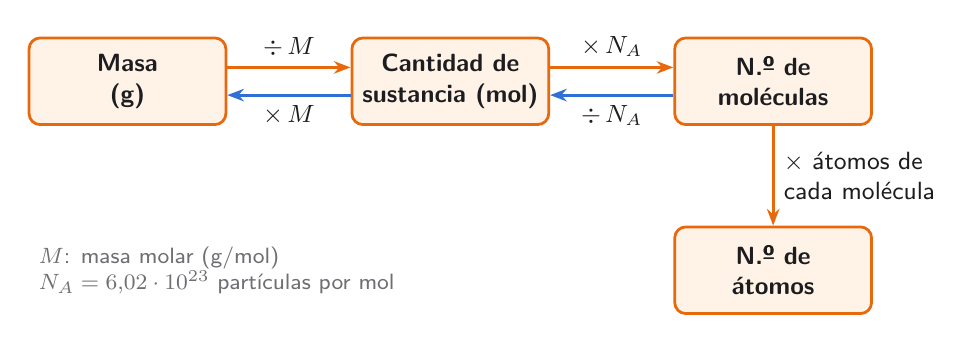
\begin{tikzpicture}
\tikzset{caja/.style={draw=nar,fill=hielo,line width=1pt,rounded corners=4pt,minimum width=2.5cm,minimum height=1.1cm,align=center,font=\sffamily\small\bfseries,text=tinta},
  fl/.style={-{Stealth[length=6pt]},line width=1.1pt},et/.style={font=\sffamily\small,text=tinta}}
\node[caja] (m) at (0,0) {Masa\\(g)};
\node[caja] (n) at (4.1,0) {Cantidad de\\sustancia (mol)};
\node[caja] (p) at (8.2,0) {N.º de\\moléculas};
\node[caja] (a) at (8.2,-2.4) {N.º de\\átomos};
\draw[fl,nar] ([yshift=5pt]m.east) -- node[et,above] {$\div\, M$} ([yshift=5pt]n.west);
\draw[fl,azul] ([yshift=-5pt]n.west) -- node[et,below] {$\times\, M$} ([yshift=-5pt]m.east);
\draw[fl,nar] ([yshift=5pt]n.east) -- node[et,above] {$\times\, N_A$} ([yshift=5pt]p.west);
\draw[fl,azul] ([yshift=-5pt]p.west) -- node[et,below] {$\div\, N_A$} ([yshift=-5pt]n.east);
\draw[fl,nar] (p.south) -- node[et,right,align=left] {$\times$ átomos de\\ cada molécula} (a.north);
\node[font=\sffamily\footnotesize,text=gris,align=left,anchor=west] at (-1.25,-2.4) {$M$: masa molar (g/mol)\\ $N_A = 6{,}02\cdot 10^{23}$ partículas por mol};
\end{tikzpicture}
\end{document}
